\section{Spatio-Temporal Epidemiological Modeler (STEM)}

For this research, the Spatio-temporal Epidemiological Modeler (STEM) distributed by IBM through the Eclipse foundation is used to see the visualization of the gathered data \cite{StemIBM}. STEM acts as a simulator of how diseases spread throughout an area, and through using this tool, the collection and analysis of data is made easier \cite{StemIBM}. Through using STEM's default sets of epidemiology setups, it can help in giving the basis for the study of how outbreaks of the chosen diseases can be forecasted and mitigated.

STEM can handle custom experiments using different parameters. Developers can change a simulation's settings from the triggers of diseases, up to policies local to a country \cite{StemIBM}. This is important for the research since the basis of the simulation is the gathered data from Twitter \cite{StemIBM}. The software is extensible enough to cater this for the research.

\begin{figure}[!ht]
    \centering
    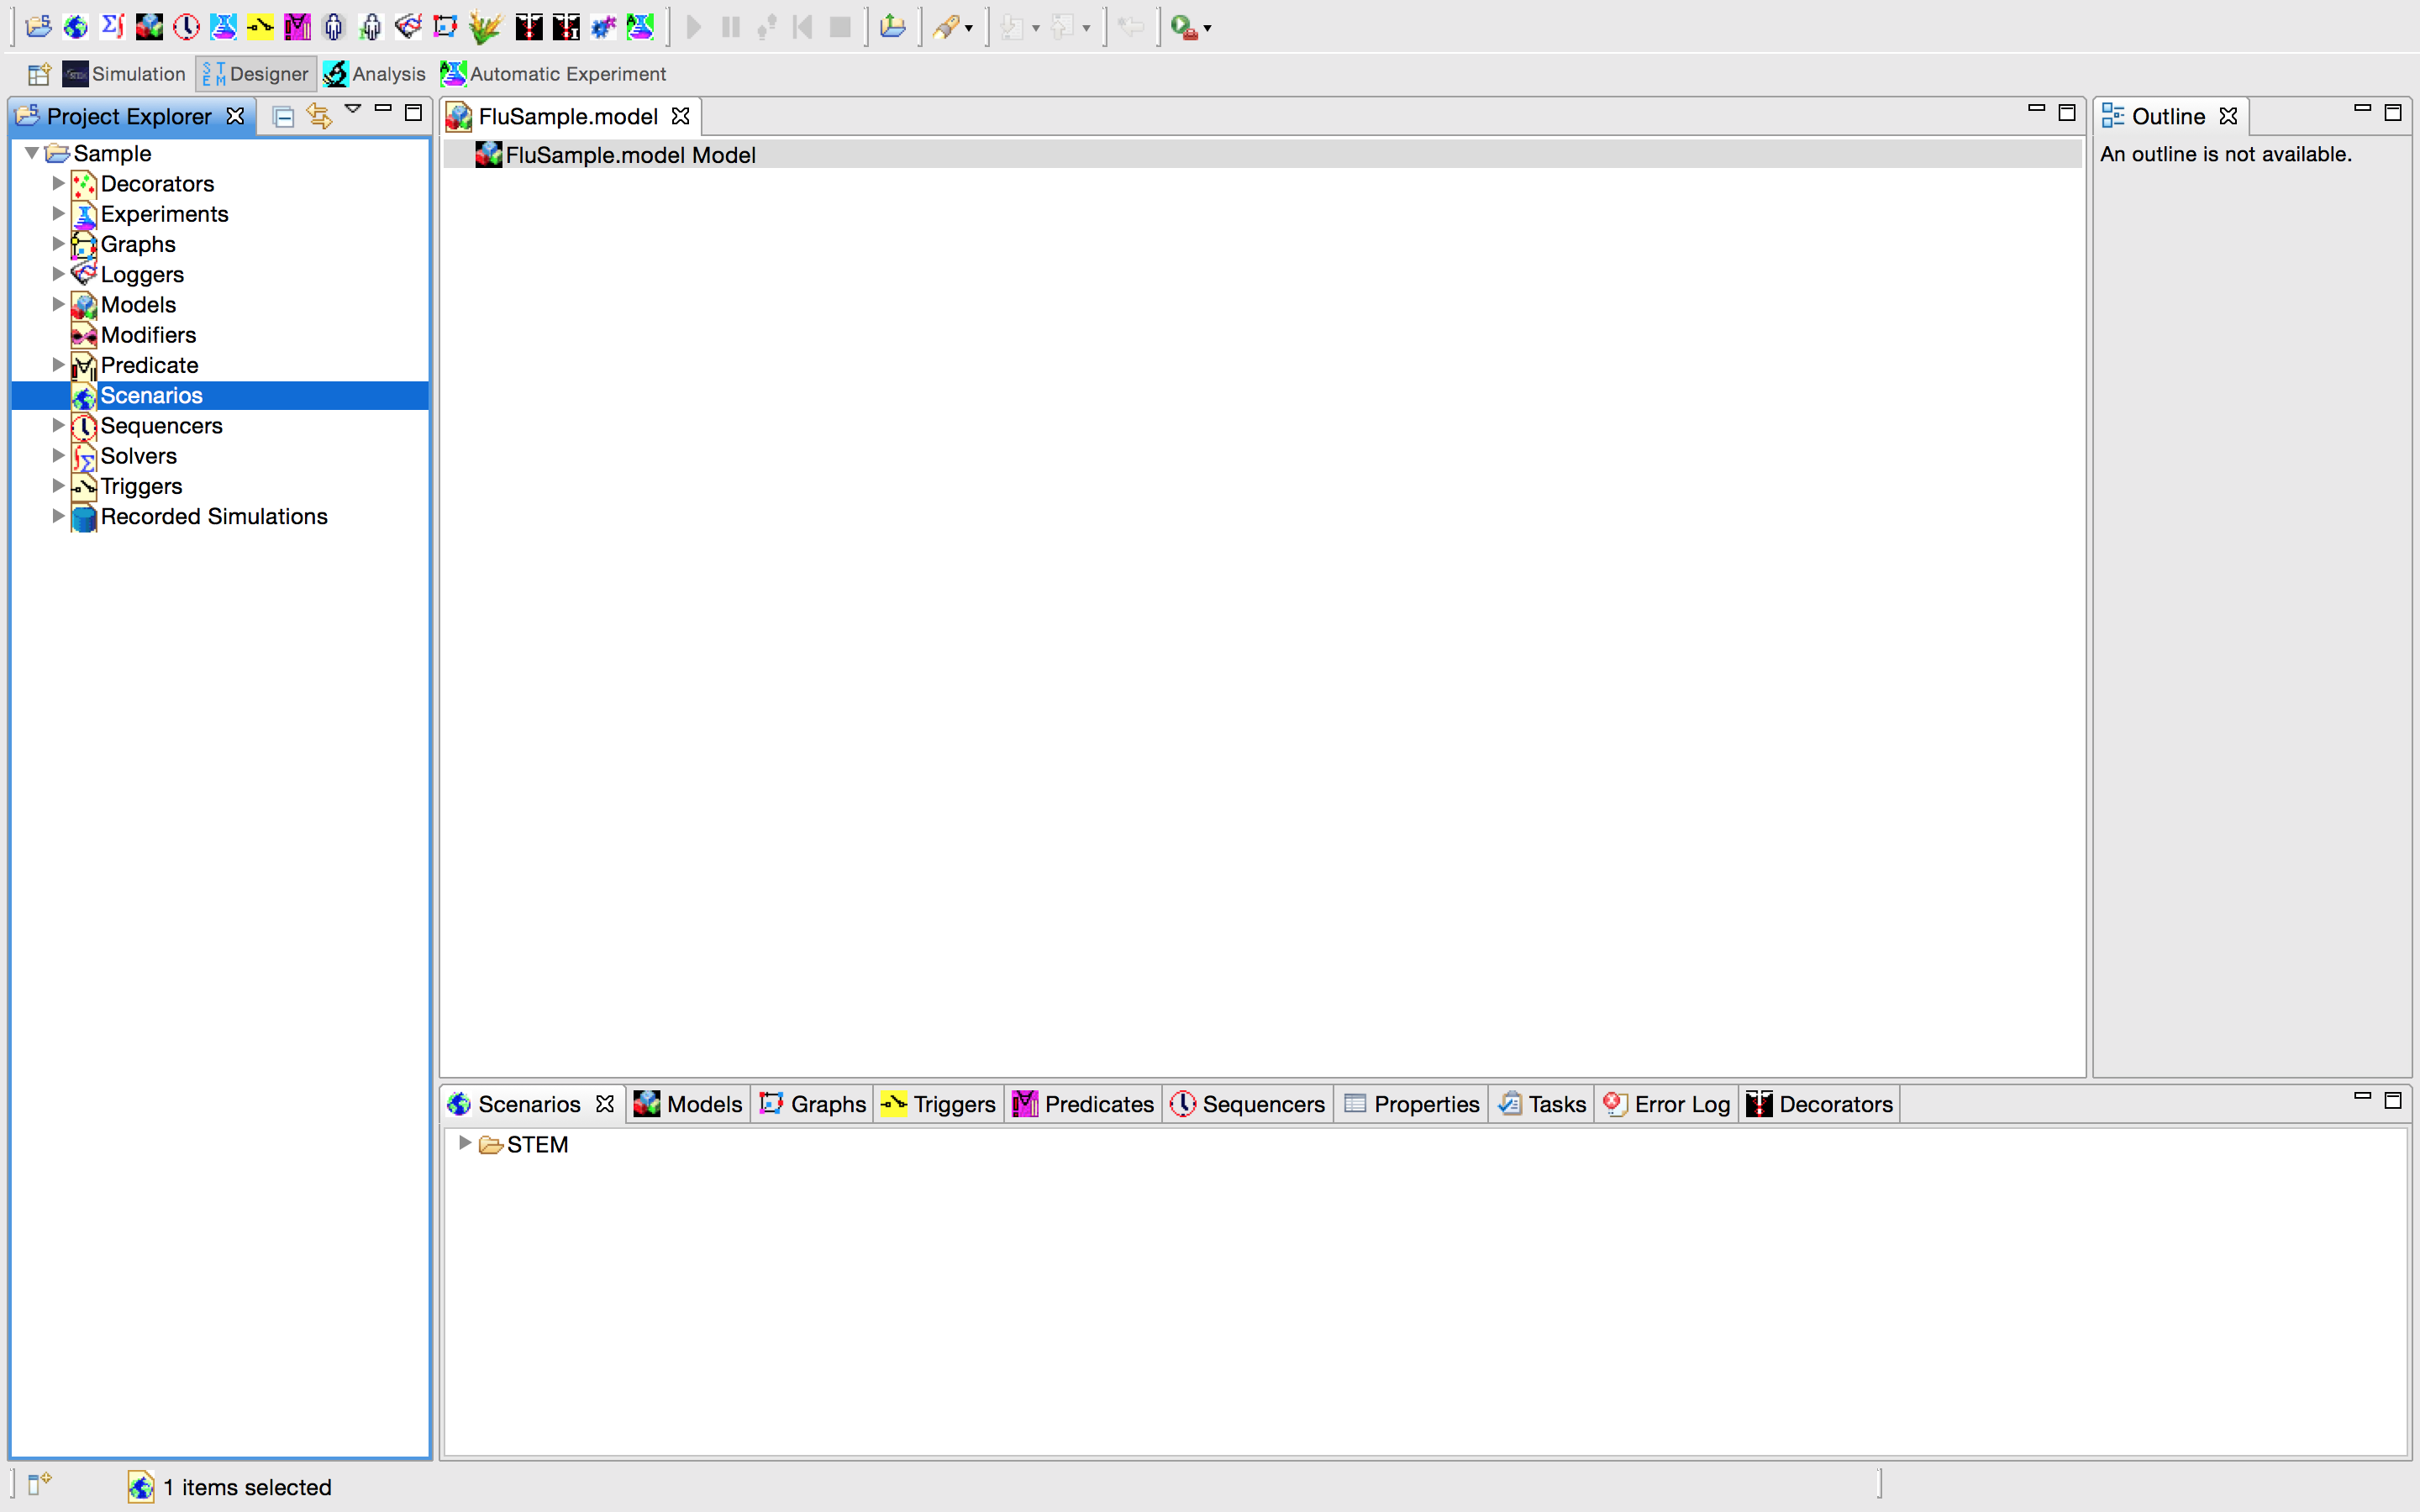
\includegraphics[width=\textwidth]{StemScreenshot}
	\caption{STEM's Integrated Development Environment by Eclipse.}
	\label{fig:StemScreenshot}
\end{figure}

\subsection{Studies Using STEM}
A group of researchers from the IBM Almaden Research center is heavily invested in producing researches using the Spatio-Temporal Epidemiological Modeler \cite{ibmalmaden}. The group is headed by Mr. James Kaufman, one of the creators of STEM, who makes studies on the spread of infectious diseases. Two (2) of the researches they made are to be discussed. First is on Influenza focusing on the SIR model used in predicting the disease in Israel, and on Dengue that shows the different compartmental models they used in modeling the disease.

\subsubsection{Influenza}
STEM was used to create a study entitled ``A Spatiotemporal Model for Influenza'' in the year 2011 \cite{edlund2009spatiotemporal}. The data used in the study focused on a 10-year data collected from 49 locations in Israel. The aim of the project is to create a predictive model using a deterministic SIR(S) compartmental disease model to account for seasonal variation of the disease \cite{edlund2009spatiotemporal}. The Susceptible-Infectious-Recovered (SIR) compartmental model will also be used for modeling the diseases in this research, as supported by Edlund's research \cite{edlund2009spatiotemporal}. Through using this model, the population is assumed to be part of only one compartment at a certain point in time. Added to this, computations are used to adjust the predictive model from the data gathered. 

As a conclusion, it was mentioned that the model they were able to make were accurate in the first two years of prediction, with a 3\% error rate, but rapidly declined for the years after \cite{edlund2009spatiotemporal}. This shows that there are other factors that needs to be considered to be able to make a near-accurate predictive model of Influenza, and the social media abstraction may add value to this research.

\subsubsection{Dengue}
Another study led by the IBM Almaden Research Center focused on the dynamics of Dengue Fever \cite{hu2013modeling}. The research focused on combatting Dengue fever re-infection by adding disease parameters such as the presence of multiple serotypes or strains of the virus. The study proceeded using a deterministic model, disregarding realistic stochastic forces outside the modelled environment. As a conclusion, the STEM software provided the researchers a platform to act as a baseline for their model.

% ***ADD the different types of compartmental models***

\subsection{STEM Loggers}

STEM loggers stores simulation data into different formats. There are different loggers available in STEM, namely \textit{CSV Logger}, \textit{Map View Logger}, \textit{Equirectangular Map Logger}, \textit{Mercator Map Logger}, \textit{Orthographic Map Logger}, and \textit{Azimuthal Equidistant Map Logger}. Table \ref{Table:StemLogger} shows the difference among these.


\begin{table}[!htbp]
\centering
\caption{Comparison of STEM Loggers}
\label{Table:StemLogger}
\begin{tabular}{SML}
\hline
\textbf{Logger}                                                             & \textbf{Compartment Logger} & Description                                                                                                                                                                                                                                                                                 \\ \hline
CSV Logger                                                                  & Yes                         & Logs simulation data to a flat file using a configurable delimeter (such as a comma).,Useful for recording raw results of a STEM simulation for analysis.                                                                                                                                   \\
Map View Logger                                                             & No                          & A simple logger for visually recording STEM simulations.,Captures the current view of the STEM Map and writes it to an image file.                                                                                                                                                          \\
Map Logger (Equirectangular, Mercator, Orthographic, Azimuthal Equidistant) & Yes                         & Highly configurable image drawers for capturing STEM simulations visually using various map projections.,Creates high resolution images using specific settings independent of the current STEM Map View.,Useful for creating production-quality STEM images for print and film animations. \\
\end{tabular}s
\end{table}


For this research, the focus will be on the CSV logger. This contains the data that will be used for the re-creation of map using a separate tool. 


%\subsection{Extensiblity}